\documentclass[12pt,a4paper]{article}

% ─── Page Layout ───────────────────────────────────────────────────────────────
\usepackage[a4paper, margin=0.8in, headheight=14pt]{geometry}

% ─── Fonts (XeLaTeX) ───────────────────────────────────────────────────────────
\usepackage{fontspec}
\usepackage{unicode-math}
\setmainfont{TeX Gyre Pagella}
\setmonofont[Scale=0.88]{TeX Gyre Cursor}
\setmathfont{Latin Modern Math}

% ─── Packages ──────────────────────────────────────────────────────────────────
\usepackage{xcolor}
\usepackage{colortbl}
\usepackage{titlesec}
\usepackage{enumitem}
\usepackage{tabularx}
\usepackage{booktabs}
\usepackage{array}
\usepackage{amsmath}
\usepackage{tikz}
\usetikzlibrary{shapes.geometric, arrows.meta, positioning, calc, fit, decorations.pathreplacing}
\usepackage{tcolorbox}
\tcbuselibrary{skins, breakable}
\usepackage{hyperref}
\usepackage{fancyhdr}
\usepackage{graphicx}
\usepackage{microtype}
\hyphenpenalty=10000
\exhyphenpenalty=10000
\sloppy
\usepackage{caption}
\usepackage{setspace}
\usepackage{multirow}
\usepackage{tocloft}

% ─── Q&A helper ────────────────────────────────────────────────────────────────
\newcommand{\Q}[1]{\textbf{#1}\par\noindent\ignorespaces}

% ─── Colour Palette ────────────────────────────────────────────────────────────
\definecolor{myred}{RGB}{196,30,58}
\definecolor{mydark}{RGB}{30,30,50}
\definecolor{mygreen}{RGB}{14,120,80}
\definecolor{myteal}{RGB}{0,130,140}
\definecolor{myamber}{RGB}{180,100,0}
\definecolor{mypurple}{RGB}{100,30,160}
\definecolor{mygray}{RGB}{246,247,249}
\definecolor{mgframe}{RGB}{180,185,200}
\definecolor{watermark}{RGB}{145,150,170}
\definecolor{hdrred}{RGB}{250,232,235}
\definecolor{hdrgreen}{RGB}{220,244,233}
\definecolor{hdrteal}{RGB}{220,242,244}
\definecolor{hdramber}{RGB}{253,242,215}
\definecolor{hdrpurple}{RGB}{238,228,255}
\definecolor{hdrgray}{RGB}{238,240,245}
\definecolor{rowalt}{RGB}{250,251,253}

% ─── Section Formatting ────────────────────────────────────────────────────────
\titleformat{\section}
  {\large\bfseries\color{myred}}{\thesection.}{0.5em}{}
  [\vspace{1pt}{\color{myred}\rule{\linewidth}{0.8pt}}]
\titleformat{\subsection}
  {\normalsize\bfseries\color{myteal}}{\thesubsection}{0.5em}{}
\titlespacing*{\section}{0pt}{18pt}{7pt}
\titlespacing*{\subsection}{0pt}{11pt}{4pt}

% ─── Paragraph ─────────────────────────────────────────────────────────────────
\setlength{\parindent}{0pt}
\setlength{\parskip}{4pt}

% ─── TOC Styling ───────────────────────────────────────────────────────────────
\renewcommand{\cfttoctitlefont}{\large\bfseries\color{myred}}
\renewcommand{\cftaftertoctitle}{\par\noindent{\color{myred}\rule{\linewidth}{0.8pt}}}
\setlength{\cftbeforetoctitleskip}{0pt}
\setlength{\cftaftertoctitleskip}{6pt}
\renewcommand{\cftsecfont}{\normalsize\bfseries\color{mydark}}
\renewcommand{\cftsecpagefont}{\normalsize\bfseries\color{mydark}}
\renewcommand{\cftsecleader}{\cftdotfill{\cftdotsep}}
\setlength{\cftbeforesecskip}{7pt}
\renewcommand{\cftsubsecfont}{\small\color{mydark}}
\renewcommand{\cftsubsecpagefont}{\small\color{mydark}}
\setlength{\cftbeforesubsecskip}{3pt}
\setlength{\cftsubsecindent}{1.4em}

% ─── Table helpers ─────────────────────────────────────────────────────────────
\renewcommand{\arraystretch}{1.45}
\setlength{\tabcolsep}{6pt}
\arrayrulecolor{mydark}
\newcolumntype{B}[1]{>{\small\bfseries\raggedright\arraybackslash}m{#1}}
\newcolumntype{Y}{>{\small\raggedright\arraybackslash}X}
\renewcommand{\tabularxcolumn}[1]{m{#1}}

% ─── Header / Footer ───────────────────────────────────────────────────────────
\pagestyle{fancy}
\fancyhf{}
\fancyhead[L]{\small\color{myred}\textbf{PE-EC701B}\;\color{mydark}--- Satellite Communication}
\fancyhead[R]{\small\color{myteal}\textbf{Module 4 Notes}}
\fancyfoot[C]{\small\color{mydark}\thepage}
\fancyfoot[R]{\small\color{watermark}\textit{\copyright\ Biraj}}
\renewcommand{\headrulewidth}{0.5pt}
\renewcommand{\footrulewidth}{0.3pt}

% ─── Hyperref ──────────────────────────────────────────────────────────────────
\hypersetup{
  colorlinks=true, linkcolor=myteal, urlcolor=myteal,
  pdfauthor={Biraj Sarkar},
  pdftitle={PE-EC701B --- Module 4 Notes}
}

% ─── tcolorbox styles ──────────────────────────────────────────────────────────
\tcbset{
  tikzbox/.style={
    colback=mygray, colframe=mgframe, boxrule=0.6pt, arc=4pt,
    left=8pt, right=8pt, top=6pt, bottom=6pt,
    colbacktitle=mgframe, coltitle=mydark,
    fonttitle=\small\bfseries
  },
  defbox/.style={
    colback=hdrgreen, colframe=mygreen, boxrule=0.8pt, arc=4pt,
    left=9pt, right=9pt, top=6pt, bottom=6pt,
    colbacktitle=mygreen, coltitle=white,
    fonttitle=\small\bfseries
  },
  formulabox/.style={
    colback=hdrteal, colframe=myteal, boxrule=0.8pt, arc=4pt,
    left=9pt, right=9pt, top=7pt, bottom=7pt,
    colbacktitle=myteal, coltitle=white,
    fonttitle=\small\bfseries
  },
  examplebox/.style={
    colback=hdramber, colframe=myamber, boxrule=0.8pt, arc=4pt,
    left=9pt, right=9pt, top=6pt, bottom=6pt,
    colbacktitle=myamber, coltitle=white,
    fonttitle=\small\bfseries
  },
  masonbox/.style={
    colback=hdrpurple, colframe=mypurple, boxrule=0.8pt, arc=4pt,
    left=9pt, right=9pt, top=6pt, bottom=6pt,
    colbacktitle=mypurple, coltitle=white,
    fonttitle=\small\bfseries
  },
  exambox/.style={
    colback=hdrpurple, colframe=mypurple, boxrule=1pt, arc=5pt,
    left=10pt, right=10pt, top=8pt, bottom=8pt,
    colbacktitle=mypurple, coltitle=white,
    fonttitle=\bfseries,
    breakable, title after break={\textbf{Frequently Asked / Viva Questions (contd.)}}}
}
% Make all boxes breakable across pages
\tcbset{breakable}

% ─── TikZ styles ───────────────────────────────────────────────────────────────
\tikzset{
  block/.style={rectangle, draw=myteal, fill=hdrteal,
    text width=2.4cm, align=center, minimum height=0.95cm,
    font=\small, rounded corners=3pt, line width=0.7pt},
  redblock/.style={rectangle, draw=myred, fill=hdrred,
    text width=2.4cm, align=center, minimum height=0.95cm,
    font=\small, rounded corners=3pt, line width=0.7pt},
  netnode/.style={rectangle, draw=myteal, fill=hdrteal,
    text width=1.5cm, align=center, minimum height=0.8cm,
    font=\small, rounded corners=3pt, line width=0.7pt},
  sumjunc/.style={circle, draw=myamber, fill=hdramber,
    minimum size=0.62cm, font=\small, line width=0.8pt},
  snode/.style={circle, draw=mypurple, fill=hdrpurple,
    minimum size=0.55cm, font=\footnotesize, line width=0.7pt},
  arrow/.style={-Stealth, thick, color=mydark},
  redarrow/.style={-Stealth, thick, color=myred},
  line/.style={thick, color=mydark}
}

% ═══════════════════════════════════════════════════════════════════════════════
\begin{document}
% ═══════════════════════════════════════════════════════════════════════════════

\begin{center}
  {\LARGE\bfseries\color{myred} PE-EC701B --- Satellite Communication}\\[5pt]
  {\normalsize\color{mydark} Semester VII \quad$\bullet$\quad 3L:0T:0P \quad$\bullet$\quad 3 Credits}\\[3pt]
  {\normalsize\color{myteal}\textbf{Module 4 Exam Notes: Typical Phenomena in Satellite Communication}}\\[3pt]
  {\small\color{mydark} CGEC \;$|$\; B.Tech ECE (2023--27) \;$|$\; \textit{Biraj Sarkar}}
\end{center}
\vspace{2pt}
\noindent{\color{myred}\rule{\linewidth}{1.5pt}}
\vspace{2pt}

\hypersetup{linkcolor=mydark}
\tableofcontents
\hypersetup{linkcolor=myteal}
\newpage

% ===============================================================================
\section{Solar Eclipse on Satellite}
% ===============================================================================

An orbital eclipse occurs when a satellite passes through the shadow cast by the Earth (or occasionally the Moon), blocking its direct line of sight to the Sun.

\begin{tcolorbox}[defbox]
\textbf{Solar Eclipse:} The condition where Earth's shadow blocks sunlight from reaching the satellite's solar panels. For geostationary (GEO) satellites, eclipses occur twice a year during the vernal and autumnal equinoxes for a 72-day period.
\end{tcolorbox}

\subsection{Eclipse Geometry and Occurrence}
Because the Earth's axis of rotation is tilted at $23.4^\circ$, GEO satellites bypass Earth's shadow during most of the year. However, during the equinoxes (late March and late September), the Sun lies in the Earth's equatorial plane, aligning the Sun, Earth, and GEO satellites.

\begin{tcolorbox}[tikzbox, title={GEO Satellite Solar Eclipse Geometry}]
\centering
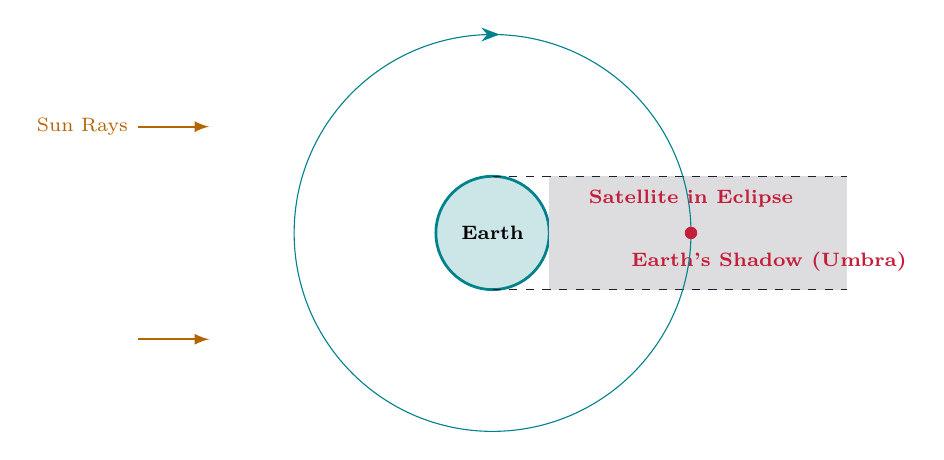
\begin{tikzpicture}[scale=0.9, every node/.style={font=\scriptsize}]
  % Sun rays (left side)
  \draw[latex-, color=myamber, thick] (-4,1.5) -- (-5,1.5) node[left] {Sun Rays};
  \draw[latex-, color=myamber, thick] (-4,-1.5) -- (-5,-1.5);
  
  % Earth (Center)
  \fill[color=myteal!20, draw=myteal, line width=1pt] (0,0) circle (0.8cm);
  \node at (0,0) {\textbf{Earth}};
  
  % Shadow boundaries (Umbra)
  \fill[color=mydark!15] (0.8,0.8) -- (5.0,0.8) -- (5.0,-0.8) -- (0.8,-0.8) -- cycle;
  \draw[dashed, color=mydark] (0,0.8) -- (5.0,0.8);
  \draw[dashed, color=mydark] (0,-0.8) -- (5.0,-0.8);
  \node[color=myred] at (3.9,-0.4) {\textbf{Earth's Shadow (Umbra)}};
  
  % Satellite Orbit Path
  \draw[color=myteal, thin] (0,0) circle (2.8cm);
  
  % Satellite entering shadow
  \coordinate (Sat) at (2.8,0);
  \fill[color=myred] (Sat) circle (2.5pt);
  \node[above=0.2cm of Sat, color=myred] {\textbf{Satellite in Eclipse}};
  
  % Direction of travel
  \draw[-Stealth, color=myteal, thick] (0,2.8) -- (0.1,2.8);
\end{tikzpicture}
\tcbset{colbacktitle=myteal, coltitle=white}
\end{tcolorbox}

\subsection{Effects of Eclipse}
\begin{itemize}[leftmargin=*, itemsep=2.5pt]
  \item \textbf{Loss of Power Generation:} The solar panels cease to generate electricity, causing the bus voltage to drop unless batteries take over.
  \item \textbf{Thermal Shock:} The temperature drops rapidly from over $+100^\circ\text{C}$ in sunlight to below $-100^\circ\text{C}$ in shadow, placing mechanical stress on components.
\end{itemize}

\subsection{Remedies}
\begin{itemize}[leftmargin=*, itemsep=2.5pt]
  \item \textbf{Secondary Battery Backup:} Lithium-Ion or $\text{Ni-H}_2$ batteries power the payload during the eclipse.
  \item \textbf{Electric Thermal Heaters:} Automatically switch on to keep sensitive transponder components at safe operating temperatures.
\end{itemize}

% ===============================================================================
\section{Sun Transit Outage}
% ===============================================================================

Sun Transit Outage is a natural phenomenon that causes temporary signal degradation when the Sun passes directly behind the satellite as seen from the receiving Earth station.

\begin{tcolorbox}[defbox]
\textbf{Sun Transit Outage:} A downlink interference event occurring when the Sun, the satellite, and the ground receiving dish align in a straight line. The Sun's intense thermal microwave emissions overwhelm the satellite's downlink signal.
\end{tcolorbox}

\subsection{Alignment Geometry}
During this alignment, the ground station antenna points directly at the satellite and, simultaneously, directly at the Sun.

\begin{tcolorbox}[tikzbox, title={Sun Transit Outage Alignment}]
\centering
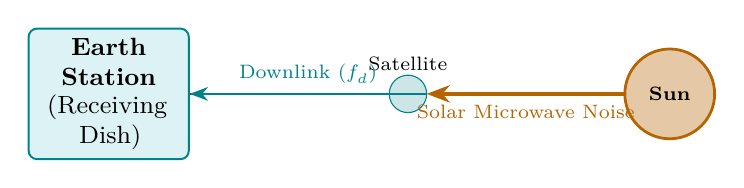
\begin{tikzpicture}[scale=0.95, every node/.style={font=\scriptsize}]
  % Sun (Right side)
  \fill[color=myamber!35, draw=myamber, line width=1pt] (5,0) circle (0.6cm);
  \node at (5,0) {\textbf{Sun}};
  
  % Satellite (Center)
  \fill[color=myteal!20, draw=myteal] (1.5,0) circle (0.25cm);
  \node at (1.5,0.4) {Satellite};
  
  % Earth Station (Left side)
  \node[block, text width=1.8cm] (es) at (-2.5,0) {\textbf{Earth Station}\\[-1pt](Receiving Dish)};
  
  % Alignment line
  \draw[color=myred, thick, dashed] (es.east) -- (1.25,0);
  \draw[arrow, color=myteal] (1.75,0) -- node[midway, above] {Downlink ($f_d$)} (es.east);
  \draw[arrow, color=myamber, line width=1.2pt] (4.4,0) -- node[midway, below, color=myamber] {Solar Microwave Noise} (1.75,0);
\end{tikzpicture}
\end{tcolorbox}

\begin{itemize}[leftmargin=*, itemsep=4pt]
  \item \textbf{Effects:} The Sun acts as an extremely high-temperature noise source ($T_{sun} > 10,000 \text{ K}$ at microwave frequencies). The antenna noise temperature ($T_{ant}$) spikes, reducing the receiver's carrier-to-noise ratio ($C/N$) to near zero, resulting in a complete communications dropout lasting up to 10 minutes.
  \item \textbf{Remedies:} Sun outages cannot be prevented physically. Ground operators mitigate the impact by:
    \begin{itemize}[leftmargin=*, itemsep=2pt, topsep=2pt]
      \item Rerouting critical traffic to adjacent satellites.
      \item Using dual-antenna setups pointed at different orbital slots.
    \end{itemize}
\end{itemize}

% ===============================================================================
\section{Doppler Frequency Shift}
% ===============================================================================

When a satellite moves relative to a terrestrial Earth station, the received frequency shifts from the transmitted frequency due to the Doppler effect.

\begin{tcolorbox}[defbox]
\textbf{Doppler Shift:} The change in apparent frequency of a received electromagnetic wave caused by relative motion between the transmitter (satellite) and receiver (ground station).
\end{tcolorbox}

\subsection{Mathematical Expression for Doppler Shift}
Let a satellite move with velocity vector $\mathbf{v}$ making an angle $\theta$ relative to the line of sight (LOS) to the Earth station.

\begin{tcolorbox}[tikzbox, title={Doppler Vector Components}]
\centering
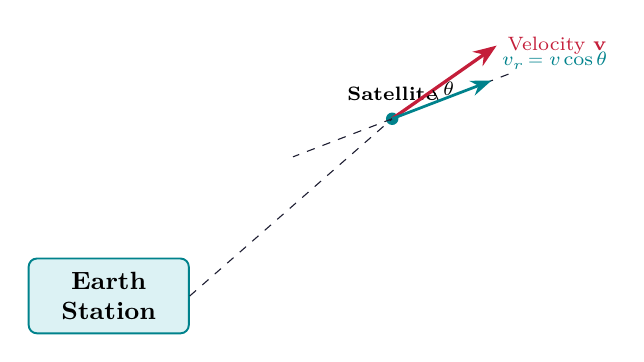
\begin{tikzpicture}[scale=0.9, every node/.style={font=\scriptsize}]
  % Earth Station
  \node[block, text width=1.8cm] (es) at (0,0) {\textbf{Earth Station}};
  
  % Satellite
  \coordinate (Sat) at (4,2.5);
  \fill[color=myteal] (Sat) circle (2.5pt);
  \node[above=0.1cm of Sat] {\textbf{Satellite}};
  
  % Velocity Vector
  \draw[arrow, color=myred, line width=1.2pt] (Sat) -- ($(Sat)+(35:1.8)$) node[right, color=myred] {Velocity $\mathbf{v}$};
  
  % Line of Sight (LOS)
  \draw[dashed, color=mydark] (es.east) -- (Sat);
  
  % Extended LOS from satellite
  \draw[dashed, color=mydark] (Sat) -- ($(Sat)+(201:1.5)$);
  \draw[dashed, color=mydark] (Sat) -- ($(Sat)+(21:1.8)$) coordinate (los_ext);
  
  % Angle theta
  \draw (Sat) +(21:0.7cm) arc (21:35:0.7cm);
  \node at ($(Sat)+(28:0.9cm)$) {$\theta$};
  
  % Projection (radial velocity)
  \draw[arrow, color=myteal, line width=1pt] (Sat) -- ($(Sat)+(21:1.5)$) node[above right, color=myteal] {$v_r = v\cos\theta$};
\end{tikzpicture}
\end{tcolorbox}

The relative radial velocity ($v_r$) along the line of sight is:
\begin{equation}
  v_r = v \cos(\theta)
\end{equation}
If $f$ is the transmitted frequency and $c$ is the speed of light, the received frequency $f'$ is:
\begin{equation}
  f' = f \left( 1 \pm \frac{v_r}{c} \right)
\end{equation}
The Doppler frequency shift ($\Delta f$) is defined as:
\begin{equation}
  \Delta f = f' - f = \pm f \frac{v_r}{c} = \pm \frac{v \cos(\theta)}{\lambda}
\end{equation}

Where:
\begin{itemize}[leftmargin=*, itemsep=3pt]
  \item $\Delta f$ = Doppler frequency shift (Hz)
  \item $f$ = Transmitted carrier frequency (Hz)
  \item $v_r = v \cos(\theta)$ = Radial velocity component (m/s)
  \item $c \approx 3 \times 10^8$ m/s = Speed of light
  \item The sign is \textbf{positive (+)} when the satellite is approaching the station.
  \item The sign is \textbf{negative (-)} when the satellite is receding from the station.
\end{itemize}

\subsection{Impact on Satcom Systems}
\begin{enumerate}[label=\textbf{\arabic*.}, leftmargin=*, itemsep=3pt]
  \item \textbf{High Frequency Vulnerability:} Since $\Delta f \propto f$, Doppler shift is severe at high frequencies (Ku and Ka bands) and in Low Earth Orbit (LEO) systems where orbital speed is extremely high ($v \approx 7.5$ km/s).
  \item \textbf{Receiver Tracking:} Receiver circuits must implement automatic frequency control (AFC) loops to track the frequency drift and maintain demodulator lock.
\end{enumerate}

% ===============================================================================
% MANDATORY QUICK REVISION PAGE
% ===============================================================================
\newpage
\begin{center}
  {\large\bfseries\color{myred} Quick Revision --- Module IV}\\[3pt]
  {\small\color{mydark} Typical Phenomena in Satellite Communication $|$ PE-EC701B}
\end{center}
\noindent{\color{myred}\rule{\linewidth}{1.2pt}}
\vspace{4pt}

\begin{tcolorbox}[formulabox, title={\textbf{Key Formulas at a Glance}}]
\renewcommand{\arraystretch}{1.9}
\begin{tabularx}{\linewidth}{B{5.0cm} X}
Doppler Frequency Shift & $\displaystyle \Delta f = \pm f \frac{v_r}{c} = \pm \frac{v_r}{\lambda}$ \\[4pt]
Relative Radial Velocity & $v_r = v \cos(\theta)$ \\[4pt]
Maximum Eclipse Duration & $t_{max} \approx 72 \text{ minutes}$ (occurs at Equinox center) \\[4pt]
Doppler Shift (Approaching) & $\displaystyle f_{received} = f_{transmitted} \left( 1 + \frac{v_r}{c} \right)$
\end{tabularx}
\end{tcolorbox}

\begin{tcolorbox}[defbox, title={\textbf{One-Line Definitions}}]
\begin{itemize}[leftmargin=*, itemsep=2.5pt, topsep=0pt]
  \item \textbf{Solar Eclipse:} Temporary blockage of sunlight to a satellite by Earth's shadow.
  \item \textbf{Equinox:} The twice-yearly period (March/September) when solar eclipses occur for GEO satellites.
  \item \textbf{Sun Transit Outage:} Alignment of ground station, satellite, and Sun, causing thermal noise outages.
  \item \textbf{Doppler Shift:} Apparent frequency deviation of a carrier wave due to relative motion.
  \item \textbf{Radial Velocity ($v_r$):} The component of satellite velocity directly along the ground station line of sight.
  \item \textbf{Umbra:} The central, completely dark portion of Earth's shadow.
  \item \textbf{AFC:} Automatic Frequency Control, used to dynamically track Doppler carrier shifts.
\end{itemize}
\end{tcolorbox}

\begin{tcolorbox}[exambox, title={\textbf{Frequently Asked / Viva Questions}}]
\begin{enumerate}[topsep=0pt, label=\textbf{Q\arabic*.}, itemsep=5pt]
  \item \Q{Why do GEO satellites experience eclipses only during equinoxes?}
    Because the Earth's orbital plane is tilted at $23.4^\circ$. Eclipses occur only when the Sun crosses the equator (during spring and autumn equinoxes), aligning the Sun, Earth, and satellite.
  \item \Q{What are the major effects of a solar eclipse on a satellite?}
    Complete loss of primary solar power generation (requiring battery operation) and severe thermal shock (temperatures drop from $+100^\circ\text{C}$ to $-100^\circ\text{C}$).
  \item \Q{How does a satellite thermal control system mitigate eclipse effects?}
    It activates electric heaters to maintain minimum operating temperatures for sensitive electronics and uses multi-layer insulation (MLI) to retain heat.
  \item \Q{Explain the physical cause of a Sun Transit Outage.}
    The Sun is a massive blackbody radiator emitting intense microwave noise. When aligned behind the satellite, this thermal noise fills the ground receiver dish beam, blocking the satellite downlink.
  \item \Q{State the duration and annual schedule of Sun Transit Outages.}
    They occur twice a year (near equinoxes) for a few consecutive days, lasting about 2 to 10 minutes per day.
  \item \Q{Derive the mathematical expression for Doppler frequency shift.}
    Let a source emit waves of period $T$. Due to radial motion $v_r$, the wave travels distance $v_r T$ per cycle. The change in apparent wavelength is $\Delta \lambda = \pm v_r / f$. Since $f = c/\lambda$, differentiating yields $\Delta f = \pm f(v_r/c)$.
  \item \Q{Under what conditions is Doppler shift maximum and zero?}
    Doppler shift is maximum when $\theta = 0^\circ$ (satellite is moving directly toward or away from the station). It is zero when $\theta = 90^\circ$ (satellite motion is perpendicular to the line of sight).
  \item \Q{Why is Doppler shift more severe in LEO satellites than in GEO satellites?}
    LEO satellites travel at extremely high speeds (~7.5 km/s) relative to Earth, creating huge radial velocity changes. GEO satellites are relatively stationary, experiencing negligible Doppler shift.
  \item \Q{Calculate the maximum Doppler shift for a LEO satellite ($v_r = 7 \text{ km/s}$) transmitting at 10 GHz.}
    $\Delta f = f \cdot (v_r/c) = 10^{10} \times (7 \times 10^3) / (3 \times 10^8) = 7 \times 10^{13} / (3 \times 10^8) \approx 233.33 \text{ kHz}$.
  \item \Q{What is the difference between Umbra and Penumbra?}
    Umbra is the inner region of the shadow where the light source is completely blocked. Penumbra is the outer region where only a portion of the light source is blocked.
  \item \Q{Why are Sun outages independent of the satellite's power status?}
    Because they are caused by external solar noise interfering with the ground receiver, not by any power loss on the satellite itself.
  \item \Q{How does a ground receiver maintain lock during a high Doppler LEO pass?}
    By using a phase-locked loop (PLL) with wide tracking bandwidth or digital frequency estimation algorithms to dynamically adjust the receiver local oscillator.
\end{enumerate}
\end{tcolorbox}

\begin{tcolorbox}[tikzbox, title={Comparison of Solar Eclipse and Sun Transit Outage}]
\renewcommand{\arraystretch}{1.4}
\par\noindent
\begin{tabularx}{\linewidth}{|B{3.2cm}|Y|Y|}
\hline
\rowcolor{hdrgray}
\textbf{Parameter} & \textbf{\color{myteal}Solar Eclipse} & \textbf{\color{myamber}Sun Transit Outage} \\
\hline
\textbf{Affected Unit} & Satellite (Spacecraft) & Ground Station (Earth Terminal) \\
\hline
\textbf{Physical Cause} & Earth blocks solar light to the satellite. & Sun aligns behind the satellite. \\
\hline
\textbf{Primary Effect} & Loss of solar power, temperature drop. & Severe thermal noise, downlink carrier loss. \\
\hline
\textbf{System Remedy} & Secondary batteries, thermal heaters. & Traffic rerouting, antenna diversity. \\
\hline
\textbf{Max Duration} & Up to 72 minutes per day. & Up to 10 minutes per day. \\
\hline
\end{tabularx}
\end{tcolorbox}

\end{document}
